Having validated the PINN approach by solving the homogeneous system, we now turn our attention toward a more advanced
inverse problem for which neural networks are particularly well-suited. In this scheme, we are given initial conditions 
along with height and velocity measurements over some unknown bathymetry which we wish to reconstruct via a PINN. 

Our test case is the inhomogeneous SWE system with a non-trivial sinusoidal bathymetry function

$$
B(x) = -\frac{1}{4} + \frac{1}{4} \cos{\left( \frac{\pi x}{5} \right)}.
$$

\noindent along with initial conditions

$$
h(x, 0) = \frac{1}{2} + \frac{2}{5} \sin{\left( \frac{\pi x}{10} \right)} \quad \text{and} \quad v(x, 0) = 0.
$$

As before, we use a neural network for the wave height and velocity with three hidden layers with 20 neurons each, along
with a second identical network (with only a single output neuron) which represents the inferred bathymetry. After 
training the network with 1000 randomly sampled height and velocity measurements over 100000 Adam iterations and 18000 
L-BFGS iterations with a learning rate $\alpha = 0.001$, we obtain a mean residual value

$$
R(\Omega) = MSE_u + MSE_f = 0.004952.
$$

\noindent again over a randomly sampled subset $\Omega$ of the computational domain. We find generally good agreement 
between the PINN and reference pseudospectral velocity (as shown in Figure \ref*{fig:inhomogeneous_swe_velocity}); the
PINN correctly captures the shape and scale of the velocity and bathymetry functions. In the velocity plot, we observe
that the PINN solution is less sharp than the reference solution near the peaks, which we attribute to the fact that 
smooth hyperbolic tangent functions comprise the PINN. Furthermore, our reference solution is near a shock; 
more research is required to characterize PINN behavior in such cases.


\begin{figure}[h]
    \centering
    \begin{subfigure}[b]{0.45\textwidth}
        \centering
        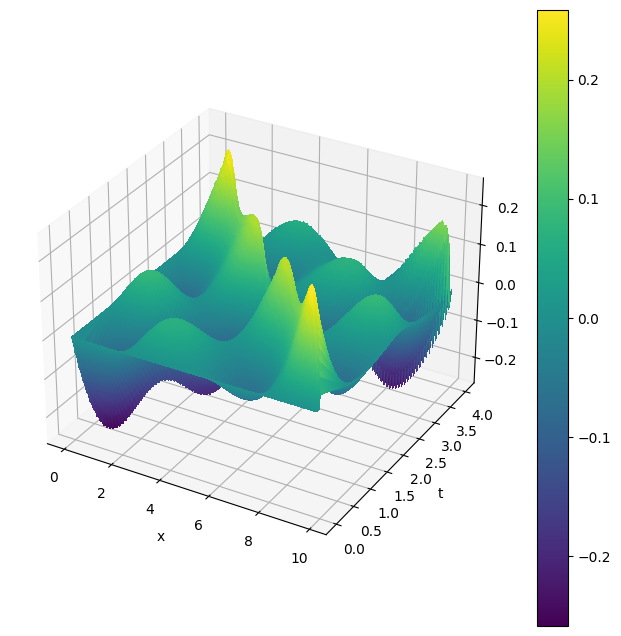
\includegraphics[width=\textwidth]{images/inhomogeneous_swe_pseudospectral_velocity.png}
        \caption{Reference wave velocity}
        \label{fig:inhomogeneous_pseudospectral_swe_velocity}
    \end{subfigure}
    \hfill
    \begin{subfigure}[b]{0.45\textwidth}
        \centering
        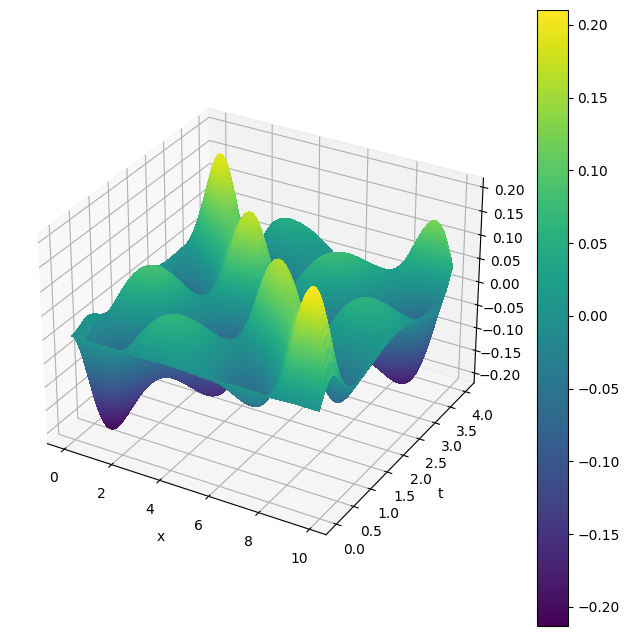
\includegraphics[width=\textwidth]{images/inhomogeneous_swe_pinn_velocity.png}
        \caption{PINN wave velocity}
        \label{fig:inhomogeneous_pinn_swe_velocity}
    \end{subfigure}
    \caption{Pseudospectral and PINN solutions for the inhomogeneous SWE system.}
    \label{fig:inhomogeneous_swe_velocity}
\end{figure}

In Figure \ref*{fig:inhomogeneous_swe_bathymetry}, we observe that the PINN recovers the shape and scale of the 
underlying bathymetry function without any prior knowledge of the reference bathymetry. While the PINN does not 
perfectly recover the original bathymetry function, we consider this a successful result and our approach validated. 
To quantify the accuracy of the neural network solution, we compute the $\ell^2$-error between values predicted by the 
trained PINN and the pseudospectral reference solution. Over the entire set of collocation points from which the 
pseudospectral solution is computed, we find this error to be $0.05647$.

\begin{figure}[h]
    \centering
    \begin{subfigure}[b]{0.45\textwidth}
        \centering
        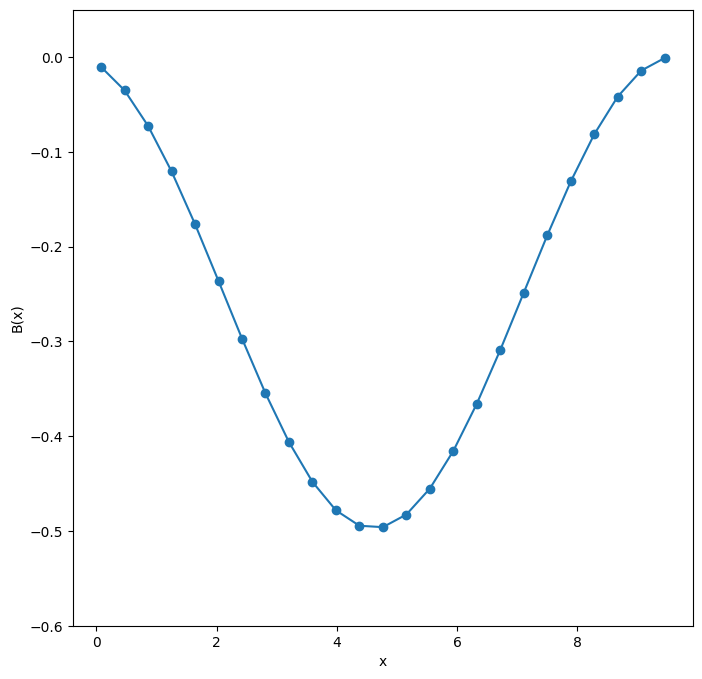
\includegraphics[width=\textwidth]{images/inhomogeneous_swe_pseudospectral_bathymetry.png}
        \caption{Reference wave bathymetry}
        \label{fig:inhomogeneous_pseudospectral_swe_bathymetry}
    \end{subfigure}
    \hfill
    \begin{subfigure}[b]{0.45\textwidth}
        \centering
        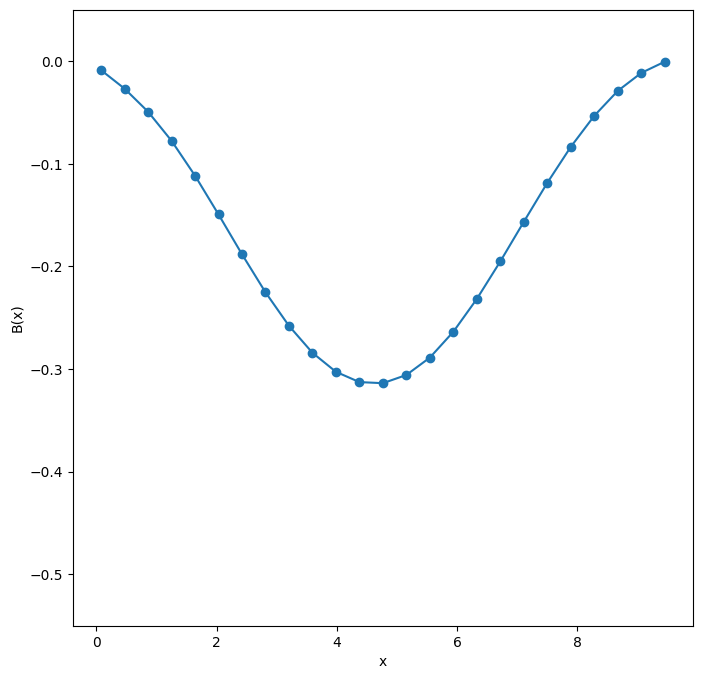
\includegraphics[width=\textwidth]{images/inhomogeneous_swe_pinn_bathymetry.png}
        \caption{Inferred PINN bathymetry}
        \label{fig:inhomogeneous_pinn_swe_bathymetry}
    \end{subfigure}
    \caption{Pseudospectral and PINN solutions for the inhomogeneous SWE system.}
    \label{fig:inhomogeneous_swe_bathymetry}
\end{figure}